\documentclass[11pt]{article}
\usepackage{mathblatt}
% gesetzt von werkzeuge/setzer.py (Sorte selbst) aus dem Lernweg 6KD
% und den Bankzeilen; Muster bau/proben/2026-10-09/hypotenuse-muster.
\usepackage{enumitem}
\usepackage{adjustbox,varwidth}
\newgeometry{a4paper,margin=18mm,top=15mm,bottom=20mm,footskip=9mm}
\pagestyle{fancy}\fancyhf{}\renewcommand{\headrulewidth}{0pt}
\fancyfoot[L]{\footnotesize\color{mbgrau}6KD \textperiodcentered{} Lösungen \textperiodcentered{} Baumdiagramm und Pfadregeln}
\fancyfoot[R]{\footnotesize\color{mbgrau}\thepage}
\setlength{\parskip}{3pt}
\renewcommand{\kreuz}[1]{\mbox{$\square$\ #1}\quad}
\newcommand{\kreuzl}[1]{\par\hangindent1.4em\hangafter1\noindent$\square$\ #1}
\newcommand{\aufg}[3]{\par\noindent\makebox[0pt][r]{#3}\begin{minipage}[t]{\linewidth}#1\end{minipage}\par}
\newcommand{\aufgg}[4]{\par\noindent\makebox[0pt][r]{#4}\begin{minipage}[t]{0.6\linewidth}\vspace{0pt}#1\end{minipage}\hfill
  \begin{minipage}[t]{0.37\linewidth}\vspace{0pt}\centering #2\end{minipage}\par}
\newcommand{\nr}[1]{\makebox[7mm][l]{\textbf{#1}}}
\newcommand{\lsg}[3]{\par\noindent\begin{minipage}[t]{9mm}\textbf{#1}\end{minipage}%
  \begin{minipage}[t]{52mm}\raggedright\bfseries\boldmath #2\end{minipage}\hspace{3mm}%
  \begin{minipage}[t]{\dimexpr\linewidth-64mm\relax}\raggedright\small #3\end{minipage}\par\vspace{4pt}}
\newlength{\kr}
\begin{document}

\noindent{\Large\bfseries Lösungen}\hspace{1em}{\color{mbgrau}Baumdiagramm und Pfadregeln}\par\smallskip
\noindent{\small Links das Ergebnis, rechts der Weg in kurzen Schritten. Stimmt dein Ergebnis nicht, such den ersten Schritt, der anders ist.}\par
\par\Needspace{25mm}\vspace{6pt}\noindent\colorbox{black!12}{\makebox[7mm]{\bfseries\strut A}}\hspace{2mm}{\bfseries Baum und Pfadregel}\par\vspace{4pt}
\lsg{1.}{Äste je $\frac{1}{2}$; $P = \frac{1}{4}$}{an jedem Ast $\frac{1}{2}$; Pfad Z – Z: $\frac{1}{2} \cdot \frac{1}{2} = \frac{1}{4}$\par\smallskip \adjustbox{max width=\linewidth,max height=4cm}{\begin{varwidth}{50cm}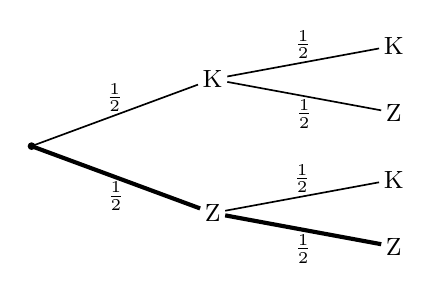
\begin{tikzpicture}[ak/.style={font=\small,inner sep=1.5pt,fill=white},wk/.style={font=\footnotesize,inner sep=1pt}]\fill (0,0) circle (1.4pt);\coordinate (s) at (0,0);\node[ak] (n0) at (2.30,0.850) {K};\node[ak] (n1) at (2.30,-0.850) {Z};\node[ak] (n00) at (4.60,1.275) {K};\node[ak] (n01) at (4.60,0.425) {Z};\node[ak] (n10) at (4.60,-0.425) {K};\node[ak] (n11) at (4.60,-1.275) {Z};\draw[line width=0.6pt] (s) -- (n0) node[wk,above,pos=0.5] {$\frac{1}{2}$};\draw[line width=1.5pt] (s) -- (n1) node[wk,below,pos=0.5] {$\frac{1}{2}$};\draw[line width=0.6pt] (n0) -- (n00) node[wk,above,pos=0.5] {$\frac{1}{2}$};\draw[line width=0.6pt] (n0) -- (n01) node[wk,below,pos=0.5] {$\frac{1}{2}$};\draw[line width=0.6pt] (n1) -- (n10) node[wk,above,pos=0.5] {$\frac{1}{2}$};\draw[line width=1.5pt] (n1) -- (n11) node[wk,below,pos=0.5] {$\frac{1}{2}$};\end{tikzpicture}\end{varwidth}}}
\lsg{2.}{$P = \frac{6}{25}$}{an jedem Punkt gelb $\frac{2}{5}$, grün $\frac{3}{5}$; Pfad gelb – grün: $\frac{2}{5} \cdot \frac{3}{5} = \frac{6}{25}$\par\smallskip \adjustbox{max width=\linewidth,max height=4cm}{\begin{varwidth}{50cm}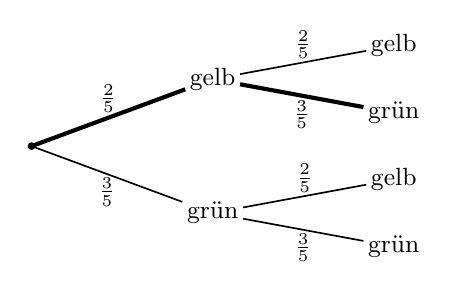
\begin{tikzpicture}[ak/.style={font=\small,inner sep=1.5pt,fill=white},wk/.style={font=\footnotesize,inner sep=1pt}]\fill (0,0) circle (1.4pt);\coordinate (s) at (0,0);\node[ak] (n0) at (2.30,0.850) {gelb};\node[ak] (n1) at (2.30,-0.850) {grün};\node[ak] (n00) at (4.60,1.275) {gelb};\node[ak] (n01) at (4.60,0.425) {grün};\node[ak] (n10) at (4.60,-0.425) {gelb};\node[ak] (n11) at (4.60,-1.275) {grün};\draw[line width=1.5pt] (s) -- (n0) node[wk,above,pos=0.5] {$\frac{2}{5}$};\draw[line width=0.6pt] (s) -- (n1) node[wk,below,pos=0.5] {$\frac{3}{5}$};\draw[line width=0.6pt] (n0) -- (n00) node[wk,above,pos=0.5] {$\frac{2}{5}$};\draw[line width=1.5pt] (n0) -- (n01) node[wk,below,pos=0.5] {$\frac{3}{5}$};\draw[line width=0.6pt] (n1) -- (n10) node[wk,above,pos=0.5] {$\frac{2}{5}$};\draw[line width=0.6pt] (n1) -- (n11) node[wk,below,pos=0.5] {$\frac{3}{5}$};\end{tikzpicture}\end{varwidth}}}
\lsg{3.}{$P = \frac{1}{8}$}{links $P(A) = \frac{1}{4}$, rechts $P(A) = \frac{2}{4}$; $\frac{1}{4} \cdot \frac{2}{4} = \frac{2}{16} = \frac{1}{8}$}
\lsg{4.}{links 3-mal A, rechts 1-mal A (oder umgekehrt)}{z.\,B. links 3-mal A, rechts 1-mal A: $\frac{3}{4} \cdot \frac{1}{4} = \frac{3}{16}$ (oder links 1-mal, rechts 3-mal A)}
\par\Needspace{25mm}\vspace{6pt}\noindent\colorbox{black!12}{\makebox[7mm]{\bfseries\strut B}}\hspace{2mm}{\bfseries Mehrere Pfade: plus}\par\vspace{4pt}
\lsg{1.}{$P = 0{,}48 = 48\,\%$}{T – D und D – T: $0{,}6 \cdot 0{,}4 + 0{,}4 \cdot 0{,}6 = 0{,}24 + 0{,}24 = 0{,}48$}
\lsg{2.}{$P = \frac{5}{8}$}{34: $\frac{1}{4} \cdot \frac{1}{4} = \frac{1}{16}$; 43: $\frac{3}{4} \cdot \frac{3}{4} = \frac{9}{16}$; zusammen $\frac{1}{16} + \frac{9}{16} = \frac{10}{16} = \frac{5}{8}$}
\lsg{3.}{$P = \frac{19}{50} = 38\,\%$}{rot – rot, blau – blau, gelb – gelb: $\frac{2}{10} \cdot \frac{2}{10} + \frac{3}{10} \cdot \frac{3}{10} + \frac{5}{10} \cdot \frac{5}{10} = \frac{4}{100} + \frac{9}{100} + \frac{25}{100} = \frac{38}{100} = \frac{19}{50}$}
\lsg{4.}{Nein; Tom gewinnt mit $\frac{11}{18}$, Mia nur mit $\frac{7}{18}$}{Nein; Mia: $\frac{3}{6} \cdot \frac{3}{6} + \frac{2}{6} \cdot \frac{2}{6} + \frac{1}{6} \cdot \frac{1}{6} = \frac{14}{36} = \frac{7}{18}$, Tom: $1 - \frac{7}{18} = \frac{11}{18}$. Tom ist im Vorteil.}
\par\Needspace{25mm}\vspace{6pt}\noindent\colorbox{black!12}{\makebox[7mm]{\bfseries\strut C}}\hspace{2mm}{\bfseries Mindestens einmal: über das Gegenteil}\par\vspace{4pt}
\lsg{1.}{$P = \frac{16}{25}$}{Gegenteil N – N: $\frac{3}{5} \cdot \frac{3}{5} = \frac{9}{25}$; $1 - \frac{9}{25} = \frac{16}{25}$}
\lsg{2.}{$\frac{5}{9}$}{Gegenteil zweimal Rot: $\frac{2}{3} \cdot \frac{2}{3} = \frac{4}{9}$, also $1 - \frac{4}{9} = \frac{5}{9}$. Nicht $\frac{1}{9}$ – das wäre nur zweimal Blau.}
\lsg{3.}{$P = \frac{7}{9}$}{rot gerade $\frac{4}{6}$, blau gerade $\frac{2}{6}$; zweimal gerade: $\frac{4}{6} \cdot \frac{2}{6} = \frac{8}{36}$; $1 - \frac{8}{36} = \frac{28}{36} = \frac{7}{9}$}
\lsg{4.}{Nein; $\frac{11}{36}$ statt $\frac{12}{36}$, um $\frac{1}{36}$ zu hoch}{Nein; $1 - \frac{5}{6} \cdot \frac{5}{6} = 1 - \frac{25}{36} = \frac{11}{36}$. Ben sagt $\frac{1}{3} = \frac{12}{36}$, er liegt um $\frac{1}{36}$ zu hoch (zweimal 6 hat er doppelt gezählt).}
\par\Needspace{25mm}\vspace{6pt}\noindent\colorbox{black!12}{\makebox[7mm]{\bfseries\strut D}}\hspace{2mm}{\bfseries Drei Stufen}\par\vspace{4pt}
\lsg{1.}{$P = \frac{1}{64}$}{ein Pfad: $\frac{1}{4} \cdot \frac{1}{4} \cdot \frac{1}{4} = \frac{1}{64}$}
\lsg{2.}{$P = \frac{125}{216} \approx 57{,}9\,\%$}{an jedem Punkt 6 $\frac{1}{6}$, k $\frac{5}{6}$; Pfad k – k – k: $\frac{5}{6} \cdot \frac{5}{6} \cdot \frac{5}{6} = \frac{125}{216}$\par\smallskip \adjustbox{max width=\linewidth,max height=4cm}{\begin{varwidth}{50cm}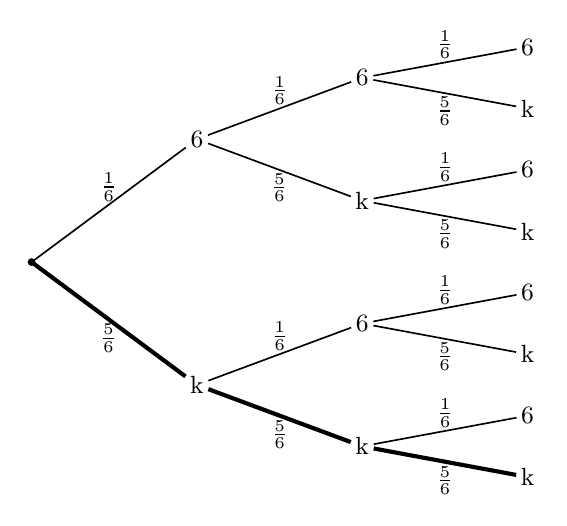
\begin{tikzpicture}[ak/.style={font=\small,inner sep=1.5pt,fill=white},wk/.style={font=\footnotesize,inner sep=1pt}]\fill (0,0) circle (1.4pt);\coordinate (s) at (0,0);\node[ak] (n0) at (2.10,1.560) {6};\node[ak] (n1) at (2.10,-1.560) {k};\node[ak] (n00) at (4.20,2.340) {6};\node[ak] (n01) at (4.20,0.780) {k};\node[ak] (n10) at (4.20,-0.780) {6};\node[ak] (n11) at (4.20,-2.340) {k};\node[ak] (n000) at (6.30,2.730) {6};\node[ak] (n001) at (6.30,1.950) {k};\node[ak] (n010) at (6.30,1.170) {6};\node[ak] (n011) at (6.30,0.390) {k};\node[ak] (n100) at (6.30,-0.390) {6};\node[ak] (n101) at (6.30,-1.170) {k};\node[ak] (n110) at (6.30,-1.950) {6};\node[ak] (n111) at (6.30,-2.730) {k};\draw[line width=0.6pt] (s) -- (n0) node[wk,above,pos=0.5] {$\frac{1}{6}$};\draw[line width=1.5pt] (s) -- (n1) node[wk,below,pos=0.5] {$\frac{5}{6}$};\draw[line width=0.6pt] (n0) -- (n00) node[wk,above,pos=0.5] {$\frac{1}{6}$};\draw[line width=0.6pt] (n0) -- (n01) node[wk,below,pos=0.5] {$\frac{5}{6}$};\draw[line width=0.6pt] (n1) -- (n10) node[wk,above,pos=0.5] {$\frac{1}{6}$};\draw[line width=1.5pt] (n1) -- (n11) node[wk,below,pos=0.5] {$\frac{5}{6}$};\draw[line width=0.6pt] (n00) -- (n000) node[wk,above,pos=0.5] {$\frac{1}{6}$};\draw[line width=0.6pt] (n00) -- (n001) node[wk,below,pos=0.5] {$\frac{5}{6}$};\draw[line width=0.6pt] (n01) -- (n010) node[wk,above,pos=0.5] {$\frac{1}{6}$};\draw[line width=0.6pt] (n01) -- (n011) node[wk,below,pos=0.5] {$\frac{5}{6}$};\draw[line width=0.6pt] (n10) -- (n100) node[wk,above,pos=0.5] {$\frac{1}{6}$};\draw[line width=0.6pt] (n10) -- (n101) node[wk,below,pos=0.5] {$\frac{5}{6}$};\draw[line width=0.6pt] (n11) -- (n110) node[wk,above,pos=0.5] {$\frac{1}{6}$};\draw[line width=1.5pt] (n11) -- (n111) node[wk,below,pos=0.5] {$\frac{5}{6}$};\end{tikzpicture}\end{varwidth}}}
\lsg{3.}{$P = 0{,}384 = 38{,}4\,\%$}{T – T – D, T – D – T, D – T – T: $3 \cdot 0{,}8 \cdot 0{,}8 \cdot 0{,}2 = 3 \cdot 0{,}128 = 0{,}384$}
\lsg{4.}{Spiel A: $40\,\%$ gegen $35{,}2\,\%$}{Spiel A. A: $\frac{2}{5} = 40\,\%$; B: genau zwei Sterne $3 \cdot \frac{2}{5} \cdot \frac{2}{5} \cdot \frac{3}{5} = \frac{36}{125}$, drei Sterne $\frac{2}{5} \cdot \frac{2}{5} \cdot \frac{2}{5} = \frac{8}{125}$, zusammen $\frac{36}{125} + \frac{8}{125} = \frac{44}{125} = 35{,}2\,\%$.}
\par\Needspace{25mm}\vspace{6pt}\noindent\colorbox{black!12}{\makebox[7mm]{\bfseries\strut T}}\hspace{2mm}{\bfseries Probetest}\par\vspace{4pt}
\lsg{1.}{$P = \frac{1}{9}$}{grün: g $\frac{2}{6}$, u $\frac{4}{6}$; gelb an beiden Punkten: g $\frac{5}{6}$, u $\frac{1}{6}$; Pfad u – u: $\frac{4}{6} \cdot \frac{1}{6} = \frac{4}{36} = \frac{1}{9}$\par\smallskip \adjustbox{max width=\linewidth,max height=4cm}{\begin{varwidth}{50cm}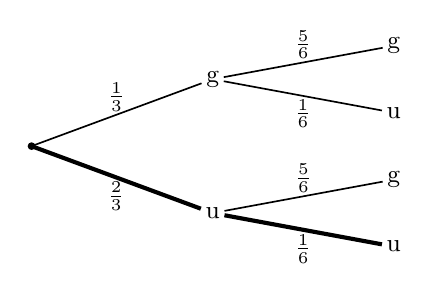
\begin{tikzpicture}[ak/.style={font=\small,inner sep=1.5pt,fill=white},wk/.style={font=\footnotesize,inner sep=1pt}]\fill (0,0) circle (1.4pt);\coordinate (s) at (0,0);\node[ak] (n0) at (2.30,0.850) {g};\node[ak] (n1) at (2.30,-0.850) {u};\node[ak] (n00) at (4.60,1.275) {g};\node[ak] (n01) at (4.60,0.425) {u};\node[ak] (n10) at (4.60,-0.425) {g};\node[ak] (n11) at (4.60,-1.275) {u};\draw[line width=0.6pt] (s) -- (n0) node[wk,above,pos=0.5] {$\frac{1}{3}$};\draw[line width=1.5pt] (s) -- (n1) node[wk,below,pos=0.5] {$\frac{2}{3}$};\draw[line width=0.6pt] (n0) -- (n00) node[wk,above,pos=0.5] {$\frac{5}{6}$};\draw[line width=0.6pt] (n0) -- (n01) node[wk,below,pos=0.5] {$\frac{1}{6}$};\draw[line width=0.6pt] (n1) -- (n10) node[wk,above,pos=0.5] {$\frac{5}{6}$};\draw[line width=1.5pt] (n1) -- (n11) node[wk,below,pos=0.5] {$\frac{1}{6}$};\end{tikzpicture}\end{varwidth}}}
\lsg{2.}{$\frac{1}{2}$}{rot – weiß $\frac{2}{5} \cdot \frac{1}{2} = \frac{2}{10}$, weiß – rot $\frac{3}{5} \cdot \frac{1}{2} = \frac{3}{10}$; zusammen $\frac{5}{10} = \frac{1}{2}$}
\lsg{3.}{$P = \frac{39}{64} \approx 60{,}9\,\%$}{Gegenteil zweimal nicht Grün: $\frac{5}{8} \cdot \frac{5}{8} = \frac{25}{64}$; $1 - \frac{25}{64} = \frac{39}{64} \approx 60{,}9\,\%$}
\lsg{4.}{$P = \frac{13}{125} = 10{,}4\,\%$}{an jedem Punkt G $\frac{1}{5}$, N $\frac{4}{5}$; genau zweimal: $3 \cdot \frac{1}{5} \cdot \frac{1}{5} \cdot \frac{4}{5} = \frac{12}{125}$, dreimal: $\frac{1}{125}$; zusammen $\frac{12}{125} + \frac{1}{125} = \frac{13}{125} = 10{,}4\,\%$\par\smallskip \adjustbox{max width=\linewidth,max height=4cm}{\begin{varwidth}{50cm}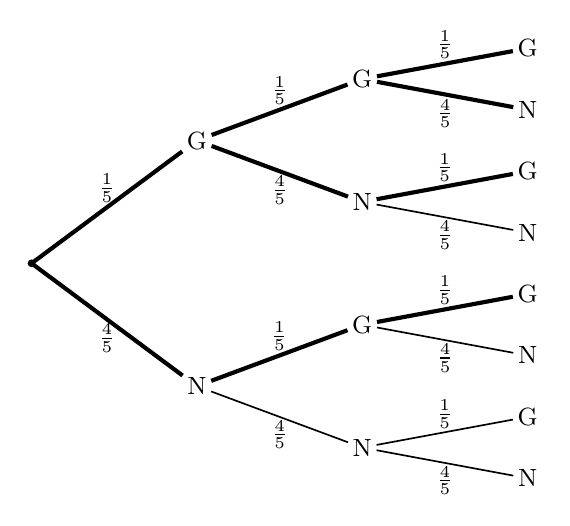
\begin{tikzpicture}[ak/.style={font=\small,inner sep=1.5pt,fill=white},wk/.style={font=\footnotesize,inner sep=1pt}]\fill (0,0) circle (1.4pt);\coordinate (s) at (0,0);\node[ak] (n0) at (2.10,1.560) {G};\node[ak] (n1) at (2.10,-1.560) {N};\node[ak] (n00) at (4.20,2.340) {G};\node[ak] (n01) at (4.20,0.780) {N};\node[ak] (n10) at (4.20,-0.780) {G};\node[ak] (n11) at (4.20,-2.340) {N};\node[ak] (n000) at (6.30,2.730) {G};\node[ak] (n001) at (6.30,1.950) {N};\node[ak] (n010) at (6.30,1.170) {G};\node[ak] (n011) at (6.30,0.390) {N};\node[ak] (n100) at (6.30,-0.390) {G};\node[ak] (n101) at (6.30,-1.170) {N};\node[ak] (n110) at (6.30,-1.950) {G};\node[ak] (n111) at (6.30,-2.730) {N};\draw[line width=1.5pt] (s) -- (n0) node[wk,above,pos=0.5] {$\frac{1}{5}$};\draw[line width=1.5pt] (s) -- (n1) node[wk,below,pos=0.5] {$\frac{4}{5}$};\draw[line width=1.5pt] (n0) -- (n00) node[wk,above,pos=0.5] {$\frac{1}{5}$};\draw[line width=1.5pt] (n0) -- (n01) node[wk,below,pos=0.5] {$\frac{4}{5}$};\draw[line width=1.5pt] (n1) -- (n10) node[wk,above,pos=0.5] {$\frac{1}{5}$};\draw[line width=0.6pt] (n1) -- (n11) node[wk,below,pos=0.5] {$\frac{4}{5}$};\draw[line width=1.5pt] (n00) -- (n000) node[wk,above,pos=0.5] {$\frac{1}{5}$};\draw[line width=1.5pt] (n00) -- (n001) node[wk,below,pos=0.5] {$\frac{4}{5}$};\draw[line width=1.5pt] (n01) -- (n010) node[wk,above,pos=0.5] {$\frac{1}{5}$};\draw[line width=0.6pt] (n01) -- (n011) node[wk,below,pos=0.5] {$\frac{4}{5}$};\draw[line width=1.5pt] (n10) -- (n100) node[wk,above,pos=0.5] {$\frac{1}{5}$};\draw[line width=0.6pt] (n10) -- (n101) node[wk,below,pos=0.5] {$\frac{4}{5}$};\draw[line width=0.6pt] (n11) -- (n110) node[wk,above,pos=0.5] {$\frac{1}{5}$};\draw[line width=0.6pt] (n11) -- (n111) node[wk,below,pos=0.5] {$\frac{4}{5}$};\end{tikzpicture}\end{varwidth}}}
\lsg{5.}{6 rote Kugeln}{$\frac{6}{10} \cdot \frac{6}{10} = \frac{36}{100} = 36\,\%$}
\end{document}
